Các mẫu     kỹ thuật được sử dụng để lập mô hình và hiện thực hóa  các thành phần riêng lẻ của hệ thống microservices.  Các mẫu     kỹ thuật  tập trung    mô hình hóa miền và triển khai logic nghiệp vụ trong lập trình.




 

Các yếu tố  các mẫu     kỹ thuật  bao gồm:





\begin{itemize}
\item Muc1  
\item Muc1  
\item Muc1  
\item Muc1  
\item Muc1  
\item Muc1  
\item Muc1  
\item Muc1  
\item Muc1  
\item Muc2  
\end{itemize}





\begin{figure}[H]

    \centering
    
    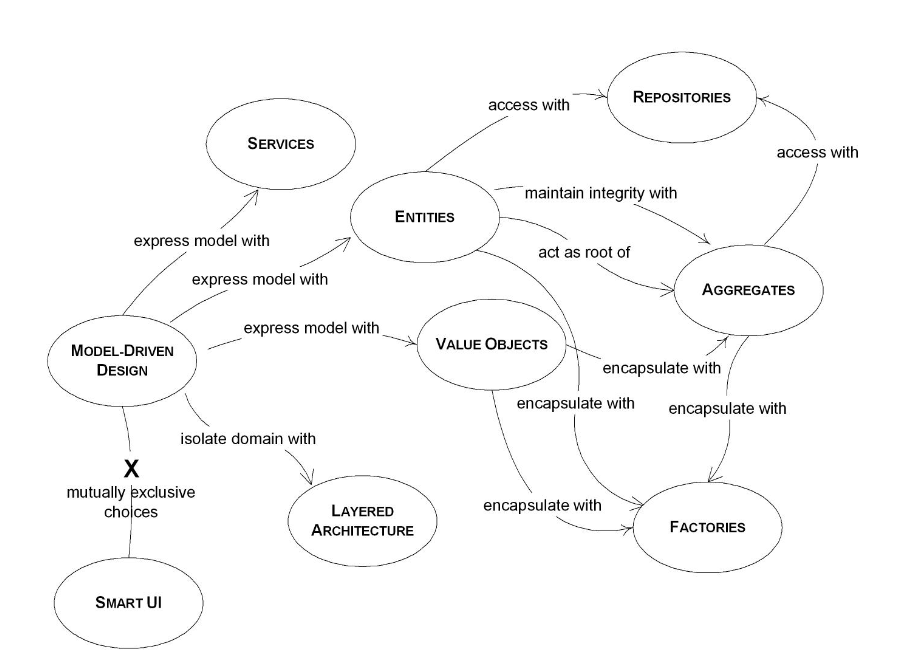
\includegraphics[scale = 0.8]{pictures/cac_mau_ky_thuat/temp.png}
    
    \caption{vvn20206205}
    
    \end{figure}
    

  

%!<! - - $ Vẽ lại sau: - - >

%!<! - - $ Vẽ lại sau: - - >

%!<! - - $ Vẽ lại sau: - - >

%!<! - - $ Vẽ lại sau: - - >

%!<! - - $ Vẽ lại sau: - - >

%!<! - - $ Vẽ lại sau: - - >

%!<! - - $ Vẽ lại sau: - - >

%!<! - - $ Vẽ lại sau: - - >

%!<! - - $ Vẽ lại sau: - - >

%!<! - - $ Vẽ lại sau: - - >

%!<! - - $ Vẽ lại sau: - - >

%!<! - - $ Vẽ lại sau: - - >

%!<! - - $ Vẽ lại sau: - - >